\documentclass[/%
a4paper,%
10pt,%
oneside,%
DIV18,
headsepline,         % Trennungslinie fuer Kopfzeile
plainheadsepline,
footsepline,         % Trennungslinie fuer Fußzeile
plainfootsepline,
%appendixprefix,
%automark,%
bibtotoc,%
liststotoc,%
BCOR12mm,%
halfparskip,%
openany,%
]{scrartcl}
\usepackage[utf8]{inputenc}
\title{Geany\LaTeX -- A \LaTeX plugin for Geany \\[1.5ex] \normalsize Version 0.4}
\author{Frank Lanitz \\ \small{frank@frank.uvena.de}}
\date{\today}
\usepackage[english]{babel}
\usepackage{listings,color}
\usepackage{courier}
\usepackage{tikz}
\lstset{basicstyle=\ttfamily\scriptsize}
\lstset{showspaces=false}
\lstset{showtabs=false}
\lstset{showstringspaces=false}
\lstset{keywordstyle=\bfseries}
\lstset{tabsize=4}
\lstset{frameround=ffff}
\lstset{extendedchars=true}
\lstset{stringstyle=\ttfamily}
\lstset{commentstyle=\ttfamily}
\lstset{backgroundcolor=\color[rgb]{0.92,0.92,0.92}}
%\lstset{numbers=left, numberstyle=\tiny, stepnumber=1, numbersep=5pt}
\lstset{captionpos=b}
\lstset{frame=single}

\begin{document}
\maketitle

\tableofcontents
\newpage

\section{About the plugin}

Geany\LaTeX\ is a little plugin to improve support of LaTeX at Geany. It
implements a couple of maybe useful functions:
\begin{itemize}
	\item Wizard to create new LaTeX documents in a fast and easy way
	 	  with a bunch of templates available
	\item A front end for add labels \textbackslash label{} and refs
	 	  \textbackslash ref{} and \textbackslash pageref{}
   		  with getting suggestion from aux file of document
	\item Inserting special characters through menu
	\item Help entering the right field for bibTeX entries by
		  providing templates
	\item Easy inserting formatings like \textbackslash texttt{}
		  through menu
	\item Support on inserting environments
	\item Shortcuts for insertings \textbackslash item and
		  \textbackslash newline
\end{itemize}


\section{Requirements}

For compiling the plugin yourself, you will need the GTK (>= 2.6.0)
libraries and header files. You will also need its dependency
libraries and header files, such as Pango, Glib and ATK. All these
files are available at http://www.gtk.org.

And obviously, you will need have Geany installed. If you have Geany
installed from the sources, you should be ready to go. If you used a
prepared package e.g. from your distribution you probably need to
install an additional package, this might be called geany-dev or
geany-devel. Please note that in order to compile and use this plugin,
you need Geany 0.16 or later (Geany Plugin API v130 or higher).

Furthermore you need, of course, a C compiler and the Make tool. The
GNU versions of these tools are recommended. Also there should be a
working \LaTeX-environment on your System.


\section{Installation}
Compiling and installing the code is done by the following three
commands:

\begin{figure}[h!]
\begin{lstlisting}
$ ./configure
$ make
$ make install %$
\end{lstlisting}
\end{figure}

For more configuration details run \texttt{./configure --help}

If there are any errors during compilation, check your build environment
and try to find the error, otherwise contact one of the authors\footnote{Contact data can be found at chapter \ref{contact} page \pageref{contact}.}

\section{Usage}

After installed successfully the plugin can be laoded through
Geany's plugin manager and a new sub menu in the Tools menu
will appear. Inside the sub menu you will find entries for
functions supported by this version of the plugin.


\section{Features}

Go into more detail on some features.

\subsection{\LaTeX-Wizard}

The \LaTeX-Wizard is implementing a easy way creating a number of
default documents.
\begin{figure}[h!]
	\centering{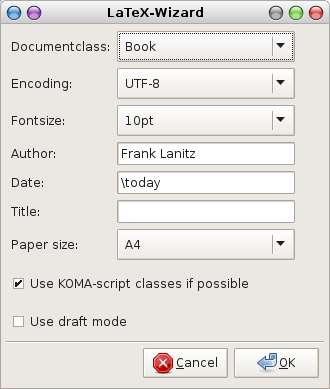
\includegraphics[height=7cm]{img/latexwizard.png}}
	\caption{\LaTeX-Wizard of version 0.3}
\end{figure}

Document types that are currently supported by the wizard are:
\begin{itemize}
	\item book
	\item report
	\item article
	\item letter
	\item presentation (\LaTeX\ beamer)
\end{itemize}

This can be set by choosing the needed entry form
\textbf{Documentclass} pulldown menu.

\textbf{Encoding} is configuring the tha packages \texttt{inputenc} to
for example \texttt{\textbackslash usepackage[utf8]\{inputenc\}} in
case of the document encoding should be UTF-8. Also it sets the
encoding Geany is using for the newly created document.

\textbf{Fontsize} as well as \textbf{Papersize} will set class option
for font/papersize of the new created document.

\textbf{Author}, \textbf{Date}, \textbf{Title} will be also passed to
the corresponding command inside the file header.

Option \textbf{Use draft mode} will add \texttt{draft} to list of
document options which allows some help during debugging of document.

Since KOMA script is quiet popular the option \textbf{Use KOMA script
if possible} allows to activate the usage of KOMA script. If this
options is activated instead of \texttt{book}, \texttt{scrbook} will
be used as document class.

The dialog can also be called by a shortcut. Please have a look onto
section \ref{kb_latex_wizard}, page \pageref{kb_latex_wizard}.


\section{Configuration}

No general configuration is needed to use the plugin. Nevertheless if
you want improve and make usage of all feature, you can define some
key bindings using Geany's key binding interface from inside the
preferences dialog.

\subsection{Keybindings}

\subsubsection*{Run LaTeX-Wizard}
\label{kb_latex_wizard}
Starts the LaTeX-Wizard for creating a new document.

\subsubsection*{Insert \textbackslash label}
Runs the dialog for inserting a new label into your document.

\subsubsection*{Insert \textbackslash ref}
Starts an dialog for easy inserting \texttt{\textbackslash ref} and
\texttt{\textbackslash pageref} into your document. The dioalog is
supporting easy parsing of aux files so it can suggest a couple of
already set labels.

\subsubsection*{Insert linebreak \textbackslash \textbackslash}
Inserts a a newline \textbackslash\textbackslash\ into the document.

\subsubsection*{Turn input replacement on/off}
A shortcut for turning input replacement on or off. When inpurt
replacement is activated special characters like \v{e} are
replaced by there \TeX\ substitute like \texttt{\textbackslash
v\{e\}}.

\subsubsection*{Replacement of special characters}
A selected text will be parsed and all known special characters will be
replaced by their \TeX substitute. This can be very useful on
importing a large amount of text into your document including
characters like "o or \frqq.

\subsubsection*{Run insert environment dialog}
Runs a dialog for easy inserting an environment. If there is some text
selected, the environment will be placed around
\begin{figure}[h!]
\begin{lstlisting}
\begin{your_environment}
	% ... selected text ...
\end{your_environment}
\end{lstlisting}
\end{figure}

In case of an empty (= no selection) an empty environment with
\begin{figure}[h!]
\begin{lstlisting}
\begin{your_environment}
...
\end{your_environment}
\end{lstlisting}
\end{figure}
empty body will inserted to the document and the curosr placed inside.

\subsubsection*{Insert \textbackslash item}
This shortcut will add an simple \textbackslash item to the document.
This can be very useful during writing of lists with a huge number of
items.


\section{Development}

You can checkout the current source code from the Subversion repository at
Sourceforge.net. Get the code from:

svn checkout
http://geany-plugins.svn.sourceforge.net/svnroot/geany-plugins/trunk/geanylatex

If you want to create a patch, please respect the license of Geany\LaTeX
as well as intellectual property of third. Patches that should be
included to the default distribution must be licensed under the same
conditions as Geany\LaTeX by the copyright owner.


\section{Known issues}

At time of the the documentation was created no issue were known.
Since this is only a snapshot, you will find more recent information
for all reported issues bug tracking system of SF at \\
http://sourceforge.net/tracker/?group\_id=222729


\section{License}


Geany\LaTeX and all its parts is distributed under the terms of the
GNU General Public License as published by the Free Software
Foundation; either version 2 of the License, or (at your option) any
later version. A copy of this license can be found in the file COPYING
included with the source code of this program. If not, you will be
able to get a copy by contacting the Free Software Foundation, Inc.,
51 Franklin Street, Fifth Floor, Boston, MA 02110-1301, USA.


\section{Bugs, questions, bugs, homepage}
\label{contact}
If you found any bugs or want to provide a patch, please contact Frank
Lanitz (frank(at)geany(dot)org). Please also do so, if you got any
questions and visiting http://frank.uvena.de/en/Geany/geanylatex/
didn't help you to figure out the answer. Visiting the website is also
a good start if you want to check for any update on this plugin.

\end{document}
